\section[Introduction]{Introduction \& Motivation}

\begin{frame}{Context}
    \begin{itemize}
        \item Mathematical models are essentially the engine driving modern engineering design.
        \item But relying on exhaustive physical testing and late-stage prototyping takes up way too much time and money.
        \item \textbf{The Goal:} We want to shift towards simulation-based design and achieve what we call "virtual certification" using Digital Twins.
    \end{itemize}
    \vspace{0.5cm}
    \begin{block}{The Big Challenge}
        When we can't afford to run endless physical tests, how can we actually trust our computational predictions?
    \end{block}
\end{frame}

\begin{frame}{Motivating Example: In-Flight Icing}
    \begin{columns}
        \begin{column}{0.5\textwidth}
            \begin{itemize}
                \item It's a severe hazard: Ice buildup completely ruins aerodynamic performance.
                \item Getting an aircraft certified by actually flying it into icing conditions is incredibly expensive.
                \item The physics are messy: We're dealing with thermodynamics, droplet dynamics, and sudden changes between different types of ice (like rime vs. glaze).
            \end{itemize}
        \end{column}
        \begin{column}{0.5\textwidth}
            \centering
            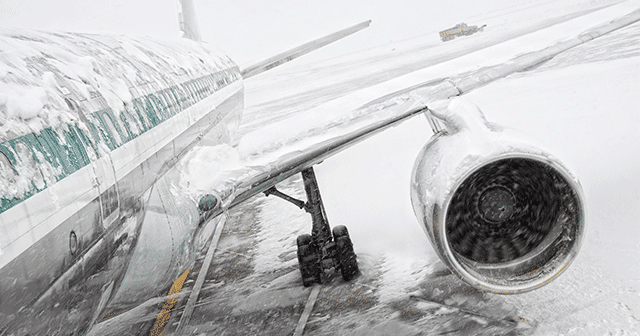
\includegraphics[width=\textwidth]{figures/wx_airplane-covered-in-ice_img-blog_0221-4139597602.png} \\
            \small{Experimental variability}
        \end{column}
    \end{columns}
\end{frame}

\begin{frame}{The Core Issue: Model Discrepancy}
    \begin{itemize}
        \item Today's numerical tools (like CFD codes for icing) lean heavily on empirical correlations and big simplifications.
        \item Because of this, we see a massive \textbf{discrepancy} between what the computer predicts and what happens in real life.
        \item Relying on just a single deterministic prediction is asking for trouble.
    \end{itemize}
    \vspace{0.5cm}
    \centering
    % 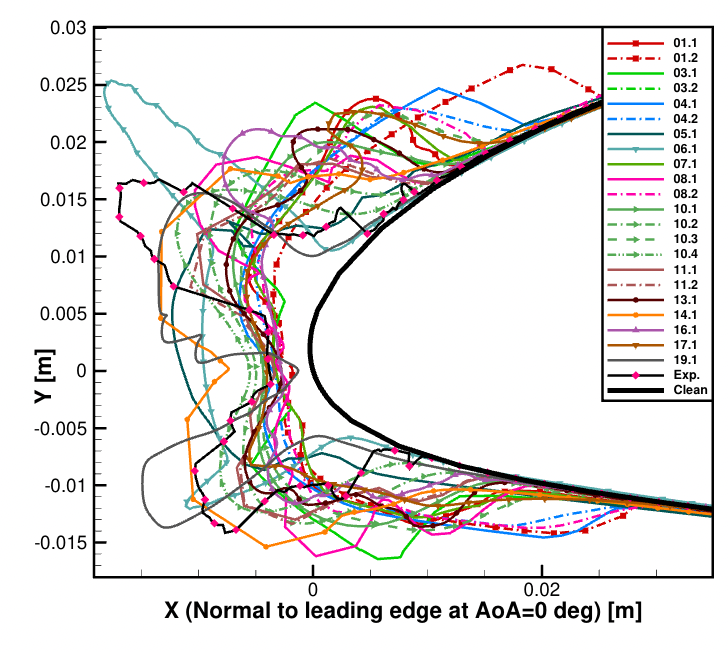
\includegraphics[width=0.6\textwidth]{figures/intro/many_shapes_2.png} \\
    \small{Numerical variability across different icing codes~\cite{many_ice_shapes_summary}}
\end{frame}

\begin{frame}{Key Bottlenecks in Uncertainty Quantification (UQ)}
    To enable reliable virtual certification, we must address two primary UQ bottlenecks:
    \vspace{0.5cm}
    \begin{enumerate}
        \item \textbf{Model Error (Calibration):} How to rigorously identify, quantify, and treat the structural discrepancy between mathematical equations and physical phenomena without incurring prohibitive computational costs?
        \vspace{0.3cm}
        \item \textbf{Discontinuous Responses (Emulation):} How to build cheap-to-evaluate surrogate models that can accurately capture abrupt physical transitions without prior expert knowledge?
    \end{enumerate}
\end{frame}

\begin{frame}{Goal of the Thesis \& Outline}
    \begin{block}{Primary Objective}
        Advance the core methodologies of Uncertainty Quantification (UQ) to unlock practical, reliable virtual certification for complex, mis-specified, and non-smooth engineering applications.
    \end{block}
    \vspace{0.5cm}
    \textbf{Outline:}
    \begin{itemize}
        \item \textbf{Part I:} Bayesian Calibration under Model Discrepancy
        \item \textbf{Part II:} Emulation of Discontinuous Responses
        \item \textbf{Conclusions}
    \end{itemize}
\end{frame}

\section{Methodological Challenges}

\begin{frame}{Aleatoric vs Epistemic Uncertainty}
    \begin{columns}
        \begin{column}{0.5\textwidth}
            
                \textbf{Aleatoric (Irreducible)}
                \begin{itemize}
                    \item Inherent variability in the physical system.
                    \item Example: Atmospheric temperature, droplet size distribution.
                    \item Must be propagated through models.
                \end{itemize}
        \end{column}
        \begin{column}{0.5\textwidth}
            
                \textbf{Epistemic (Reducible)}
                \begin{itemize}
                    \item Lack of knowledge about the system or parameters $\btheta$.
                    \item Example: Thermal conductivity, surface roughness.
                    \item Can be reduced via \textit{inference} by combining models with data $\data$.
                \end{itemize}
        \end{column}
    \end{columns}
    \vspace{0.5cm}
    \begin{block}{Bayesian Inference}
        Treats unknown parameters as random variables:
        $$ \p{\btheta \mid \data} \propto \p{\data \mid \btheta} \prior{\btheta} $$
    \end{block}
\end{frame}

\begin{frame}{The Challenge of Model Error}
    \begin{itemize}
        \item What if the physical equations are inherently flawed?
        \item The \textit{true} value of a parameter becomes ill-defined.
        \item \textbf{Objective:} Find a suitable pair of parameters $\btheta$ and model error $\bpsi$ that best explains the data.
    \end{itemize}
    \vspace{0.3cm}
    \begin{center}
        \begin{tikzpicture}
            \node[draw, rounded corners, fill=blue!10, text width=3cm, align=center] (fb) {Full Bayesian (FB) \\ Joint Inference};
            \node[draw, rounded corners, fill=red!10, text width=3cm, align=center, right=2cm of fb] (mod) {Modular \\ Sequential Inference};
            
            \draw[->, thick] (fb) -- node[above] {Curse of dimensionality} (mod);
            \node[below=0.2cm of fb, text width=3cm, align=center, font=\small] {Coherent but intractable};
            \node[below=0.2cm of mod, text width=3cm, align=center, font=\small] {Tractable but biased (False certitude)};
        \end{tikzpicture}
    \end{center}
\end{frame}

\begin{frame}{Emulation Challenges}
    \begin{itemize}
        \item Rigorous UQ requires millions of model evaluations, demanding cheap-to-evaluate \textbf{surrogate models}.
        \item \textbf{The specific issue:} Discontinuous responses (e.g., regime shifts in icing).
    \end{itemize}
    \vspace{0.3cm}
    \begin{block}{Failure of Standard Surrogates}
        \begin{itemize}
            \item Global models (like GPs or PCEs) assume smoothness.
            \item Result: Gibbs phenomenon (spurious oscillations) near discontinuities.
            \item Biased parameters and poor convergence rates.
        \end{itemize}
    \end{block}
\end{frame}
